\documentclass[letterpaper,12pt]{article}
\usepackage{tabularx} % extra features for tabular environment
\usepackage{amsmath}  % improve math presentation
\usepackage{graphicx} % takes care of graphic including machinery
\usepackage[margin=1in,letterpaper]{geometry} % decreases margins
\usepackage{cite} % takes care of citations
\usepackage[final]{hyperref} % adds hyper links inside the generated pdf file
\hypersetup{
	colorlinks=true,       % false: boxed links; true: colored links
	linkcolor=blue,        % color of internal links
	citecolor=blue,        % color of links to bibliography
	filecolor=magenta,     % color of file links
	urlcolor=blue         
}
\usepackage{blindtext}
\usepackage{mathtools}
\usepackage{tikzsymbols}

\DeclarePairedDelimiter\ceil{\lceil}{\rceil}
\DeclarePairedDelimiter\floor{\lfloor}{\rfloor}
%++++++++++++++++++++++++++++++++++++++++


\begin{document}

\title{Proyecto 1 --- Sudoku Solver}
\author{David Segura 13-11341 \& Amin Arriaga 16-10072}
\date{28 de Junio, 2020}
\maketitle

\begin{abstract}
En este proyecto aplicamos todo el contenido estudiado en la materia Diseño de Algoritmos I dictada por el profesor Ricardo Monascal. \textbf{Nota especial:} Gran reconocimiento de agradecimiento al estudiante Amin Arriaga por decidirse a cursar la materia (by D10S).
\end{abstract}


\section{Introducción}

Dado un número entero positivo $N$, un tablero de Sudoku de orden $N^2$ es una matrix de $N^2$ filas y
$N^2$ columnas, donde la matriz está dividida en $N^2$ secciones disjuntas, cada una una matriz de tamaño $N$ x $N$, el proyecto requiere que se encuentre una solución a dicho Sudoku.\\
\\
Para conseguir una respuesta al problema debemos reducir la obtención de una solución para el Sudoku a una traducción en \textbf{SAT} (\textit{Boolean Satisfiability Problem}), donde se transforman las casillas del Sudoku a una expresión booleana con variables y sin cuantificadores, para saber si hay alguna asignación de valores para sus variables que hace que la expresión sea verdadera. De esta manera si se consigue, podemos traducir esa expresión de nuevo a una solución para el Sudoku y dar el objetivo por cumplido.

\section{Desarrollo}

\subsection{Entrada}
Cada instancia será representada por una linea de texto con el siguiente formato: \\

• Un entero $N$, tal que $1 \leq N \leq 3$\\

• Un espacio en blanco\\

• Una cadena $T$ de $N^2$ números, donde $0 \leq T_i \leq N$\\

\hspace{1cm}– Si $T_i$ = 0 la casilla está vacía\\

\hspace{1cm}– Si $T_i \neq$ 0 la casilla tiene el dígito $T_i$\\
\\
Por ejemplo, la siguiente cadena representa a nuestro ejemplo de tablero de Sudoku de orden 3.\\

\footnotesize{3 000400009020980030093000840000000000200008067160300002049000650600003000000059010}\\
\\
\normalsize
La entrada del programa será un archivo con tantas líneas como instancias se quieran resolver.

\subsection{Reducción de Sudoku a SAT}

Es posible reducir cualquier instancia de Sudoku a SAT, representando el estado del tablero con variables y cláusulas de una fórmula en CNF (\textit{Forma Normal Conjuntiva}).\\
\\
Para la implementación de esta solución representaremos las casillas del tablero de Sudoku con el conjunto de variables $V = [x^1_{0,0}, ..., x^d_{i,j}, ..., x^{N^2}_{N^2-1, N^2-1}]$ con $0 \leq i, j < N^2$ y $0 < d \leq N^2$, donde $x^d_{i,j}$ ser\'a verdadera si la casilla $(i,j)$ del tablero tiene el número $d$.\\
\\
Hallamos una biyección entre $[1, N^6]$ que representan las variables booleanas en SAT y el conjunto $V$ dada por:\\

$f: V \rightarrow [1,N^6]$
\begin{equation*}
    f(i,j,d) = i \times N^4 + j \times N^2 + d \hspace{1cm} \label{eq:1} (1)
\end{equation*}\\

$f^{-1} : [1,N^6] \rightarrow V$

\begin{equation*}
    f^{-1}(x) = \left(\floor*{\frac{x}{N^4}},  \floor*{\frac{mod(x,N^4)}{N^2}}, mod(x,N^2) + 1 \right) \hspace{1cm} \label{eq:2} (2)
\end{equation*}\\
\\
Las funciones (1) y (2) las representamos en los programa \textit{sudoku\_to\_SAT.py} y \textit{SAT\_to\_sudoku.py} a través de las funciones \texttt{F} y \texttt{F\_inv} respectivamente. Dichos módulos se encargan de ejecutar la reducción de Sudoku a SAT y viceversa respectivamente, usando \texttt{F} para crear las cl\'ausulas del problema SAT a partir de la instancia de sudoku y \texttt{F\_inv} para traducir la soluci\'on del problema SAT a un tablero de sudoku.\\
\\
Estas cláusulas $C$ vienen dadas por la completitud, la unicidad, la validez y las variables instanciadas.

\begin{itemize}
	\item \textbf{Completitud:} Se crean tantas cláusulas de tamaño $N^2$ como casillas hay en el tablero, por lo tanto hay $N^4$ cl\'ausulas de completitud, cada una de la siguiente forma: \\ \\ \texttt{[F(i, j, 1, N),..., F(i, j, d, N),..., F(i, j, N$^2$, N)]} para $0 \leq i,j < N^2$, e indican que en la casilla $(i, j)$ debe haber alg\'un valor entre $1$ y $N^2$.

	\item \textbf{Unicidad:} En cada casilla no puede haber al mismo tiempo dos n\'umeros $d$ y $d'$ con $1 \leq d < d' \leq N^2$. Estas cláusuras quedarian de la siguiente forma:\\ \texttt{[-F(i, j, d, N),  -F(i, j, d', N)]} con  $0 \leq i,j < N^2$. Por lo tanto habr\'an $\left( \begin{smallmatrix} N^2 \\ 2 \end{smallmatrix} \right) \times N^4 = \frac{N^8 - N^6}{2}$ cl\'ausulas de esta tipo.
	
	\item \textbf{Instancias del sudoku:} Son las casillas ya asignadas del sudoku, los cuales diferencian cada instancia del tablero. La representación de esta cláusula viene dada de esta manera:\\ \texttt{[F(i, j, sudoku[i][j], N)]} para $0 \leq i,j < N^2$ si \texttt{sudoku[i][j] != 0}, por lo tanto habr\'an a lo sumo $N^4$ cl\'ausulas de este tipo.

	\item \textbf{Validez:} Estarán divididas en tres tipos: por filas, por columnas y por secciones. Por fila, tomaremos cada par de casillas distintas y cada dígito $d$ sólo puede estar en una de las dos, análogamente sucede con las columnas. En las secciones $k$, por cada par de casillas distintas pertenecientes a la misma, no puede haber un dígito que ocupe a ambas. Por lo tanto habr\'an $3 N^4 \left( \begin{smallmatrix} N^2 \\ 2 \end{smallmatrix} \right) = \frac{3(N^8 - N^6)}{2}$ cl\'ausulas de este tipo. Las cláusulas para esta parte son:\\

	\begin{itemize}
		\item Para las filas:
\texttt{[-F(i, j, d, N),  -F(i, j', d, N)]} para 
$$0 \leq i < N^2, \hspace{0.8cm}$$
$$\hspace{0.4mm} 0 \leq j < j'< N^2 \hspace{0.8cm} \texttt{y}$$ 
$$1 \leq d \leq N^2 \hspace{0.8cm}$$\\
		
		\item Para las columnas:
\texttt{[-F(i, j, d, N),  -F(i', j, d, N)]} para 
$$0 \leq i < i'< N^2,\hspace{1cm}$$ 
$$0 \leq j < N^2 \hspace{0.8cm} \texttt{y}$$
$$1 \leq d \leq N^2\hspace{1cm}$$\\
		
		\item Para las secciones:
\texttt{[-F(i, j, d, N),  -F(i', j', d, N)]} para 
\begin{equation*}
   N \floor*{\frac{k}{N}} \leq i \leq i' < N \floor*{\frac{k}{N}} + N \texttt{,}
\end{equation*}
\begin{equation*}
   N mod(k,N) \leq j, j' < N mod(k,N) + N \texttt{,}
\end{equation*}
$$1 \leq d \leq N^2 \hspace{1cm}$$
$$0 \leq k < N^2 \hspace{1.2cm} \texttt{y}$$
$$(i,j) \neq (i',j') \hspace{1cm}$$.\\
	\end{itemize}

\end{itemize}

Al final tendremos que solucionar una problema SAT con $|V|= N^6$ variables \hspace{0.2cm} y \hspace{0.2cm} $|C|= |completitud| + |unicidad| + |validez| + |instancia| = N^4 + \frac{N^8 - N^6}{2} + \frac{3(N^8-N^6)}{2} + I = 2N^8 - 2N^6 + N^4 + I$ cl\'ausulas, donde $ 0 \leq I = |instancia| \leq N^4$.\\ \\

La función \texttt{sudoku\_to\_SAT} recibe una matriz que representa la instancia del sudoku y retorna un string con la representación en SAT de la instancia del sudoku:

\texttt{\\
c Ejemplo de salida para sudoku\_to\_SAT\\
c \\
p cnf V C \\
v1 -v2 0\\
v3 -v4 0\\
v2 0\\
.\\
.\\
.\\}\\
La entrada de \texttt{sudoku\_to\_SAT} viene dada por la función \texttt{read\_sudoku}, la cual recibe la instancia del sudoku en string y devuelve una matriz $N \times N$, donde implementamos la extensión permitiendo que $1 \leq N \leq 6$.\\
\\
Dentro de la función \texttt{sudoku\_to\_SAT} hacemos uso de las funciones \texttt{F} y \texttt{plus}:\\

\texttt{F}: es la función (1) antes mencionada en \ref{eq:1}, usada para obtener las transformaciones correspondientes.\\

\texttt{plus}: recibe la posición de una casilla $(i,j)$, la secci\'on $k$ y el grado $N$; y retorna la posición de la siguiente casilla dentro de la misma sección $k$ mediante las siguiente formulas:

	$$ D = N \times mod(k, N) $$
   	$$i = i + \floor*{\frac{j+1}{D+N}}$$
   	$$j = mod(j+1,D+N) + D \floor*{\frac{j+1}{D+N}}$$

Esto funciona de la siguiente manera: Si el valor de la siguiente columna $j+1$ alcanza al desplazamiento por sección $D$ mas el grado del sudoku $N$, significa que debemos pasar a la siguiente fila por lo que se le aumenta 1. En caso contrario no se le suma nada. Para las columnas, el término de la izquierda se encarga que la columna no supere el desplazamiento más el grado del sudoku, que corresponderia a la última columna de la sección, más 1. Sin embargo, dejando solo este término la columna regresaría a 0 al alcanzar dicho máximo, por lo tanto, el término de la derecha notemos que es el mismo que el de $i$ multiplicado por el desplazamiento, esto significa que al superar la máxima columna, el término de la izquierda es 0, y el de la derecha es 1 por $D$, correspondiente a la primera columna de la sección.\\ \\


\textbf{Tiempo Asintóstico:}\\
Si $n$ es la dimensi\'on de la matriz del sudoku, es decir, $n = N^2$, entonces:
\begin{itemize}
	\item \texttt{sudoku\_to\_SAT} $\in O(n^4)$, debido a que estamos recorriendo una matriz ($O(N^2 \times N^2)$), comparando para cada par de casillas por fila/columna excepto consigo mismo ($O(N^2)$) para cada digito ($O(N^2)$), quedando $N^2 \times N^2 \times N^2 \times N^2 \in O((N^2)^4)$.
	\item \texttt{read\_sudoku} $\in$ O($n$), ya que debe recorrer el string de la instancia del sudoku digito por digito para asignarle su casilla correspondiente en la matriz.
	\item \texttt{F} $\in O(1)$.
	\item \texttt{plus} $\in O(1)$.\\
\end{itemize} 


\textbf{Memoria Asintótica:}\\ 
Si $n$ es la dimensi\'on de la matriz del sudoku, es decir, $n = N^2$, entonces:
\begin{itemize}
	\item \texttt{sudoku\_to\_SAT} $\in O(n^4)$, pues se almacenan todas las cl\'ausulas del sudoku, y como vimos anteriormente, hay $O(N^8) = O(n^4)$ cl\'ausulas.
	\item \texttt{read\_sudoku} $\in O(n)$.
	\item \texttt{F} $\in O(1)$.
	\item \texttt{plus} $\in O(1)$.
\end{itemize}


\subsection{SAT Solver}

El Problema de Satisfacibilidad Booleana o SAT consta de intentar hallar una asignación booleanas para las variables, que hagan que la fórmula en lógica proposicional sea satisfecha (evalúe a \textit{True}).\\

Ya con el sudoku transformado en un problema SAT en formato CNF, implementamos una función llamada \texttt{read\_SAT} que recibe el problema en el formato mencionado y retorna dos arreglos, uno de vectores que dentro del programa tratamos como \textit{V}, el cual contiene valores inicializados en $0$ para efectos más prácticos al momento de resolver el problema. No confundir el valor $0$ de una variable con \textit{False}, ya que nosotros consideramos \textit{False} como $-1$ y \textit{True} como $1$, por lo que $0$ se considera no inicializado. La longitud de este arreglo será la cantidad de variables encontradas en el problema SAT donde cada posición en el vector representará a la variable en sí. El otro arreglo que devuelve son las cláusulas que formamos al momento de traducir la instancia del sudoku.\\
\\
Con estas dos estructuras de datos formadas, pasamos a la función estrella del programa, la llamamos \texttt{laura\_SAT} \Cooley, es una función recursiva que se compone de dos funciones importantes: \texttt{update\_C} y \texttt{verify\_units}. Hablemos primero de estas dos funciones para entender el funcionamiento de \texttt{laura\_SAT}:\\

\begin{itemize}
	\item \texttt{update\_C}: esta función recibe 3 parametros, \textit{V} que corresponde a las variables y su valor lógico, \textit{C} que son las cláusulas y \textit{k} que es una variable correspondiente a la posici\'on $k-1$ de \textit{V}. El objetivo es actualizar las cláusulas con respecto a la variable \textit{k} siguiendo las siguientes reglas:
	
	\begin{itemize}
		\item Si el literal encontrado en la cláusula es \textit{False}, se elimina dicho literal.
		
		\item En caso contrario, si es \textit{True} se elimina toda la cláusula a la que pertenece.
	\end{itemize}
	
	Si al actualizar las cláusulas alguna de ellas quedó vacía, significa que se hizo una mala asignación de literales y por ende la función retorna \textit{True}, que en el ambiente de \texttt{laura\_SAT} significa que hubo conflicto, de lo contrario la actualización resulto exisota. 
	
	\item \texttt{verify\_units}: Esta función recibe las variables \textit{V} y las cláusulas \textit{C} y retorna un valor booleano que indica si hubo algún conflicto. En este método se realiza la verificación de cláusuras unitarias y en caso de haberlas actualiza las variables en consecuencia, colocándoles el mismo signo que posee en la cláusula, de esta manera se satisfacerán las clausulas unitarias, y si encuentra que ya la variable había sido asignada con el signo contrario, esta devuelve conflicto. Después que encuentra todas las cláusulas unitarias, realiza un actualización de cláusulas mediante \texttt{update\_C}, donde si da conflicto es porque se hizo una mala asignación de variables antes. 
	
	\item También está la función \texttt{search\_amin\_zero}, que dado un arreglo de variables, buscará la menor posici\'on tal que en el arreglo haya un \texttt{0}.
	
	\item \texttt{laura\_SAT}: Basada en el algoritmo de \textit{BFS}, selecciona la primera variable que aun no haya sido asignada (\texttt{search\_amin\_zero}), se le asigna el valor de \texttt{1} (\texttt{True}), se actualizan las clásulas (\texttt{update\_C}) y luego se verifica si quedaron cláusulas unitarias (\texttt{verify\_units}). En caso de no haber quedado un conflicto (alguna cláusula vacía) se verifica si a\'un quedan cl\'ausuras, si no es as\'i, significa que conseguimos una asignaci\'on de variables exitosa y retornamos la asignaci\'on actual (sustituyendo los 0 por -1) junto a \texttt{False} (que indica que no hubo conflictos). Si a\'un quedan cl\'ausulas, se realiza una llamada recursiva a \texttt{laura\_SAT} con las cl\'ausulas y variables actuales, si esta llamada retorna un arreglo junto a \texttt{False}, significa que se consigui\'o una asignaci\'on correcta de variables en una rama posterior y se retorna el mismo arreglo junto con \texttt{False}, en cambio si se retorna un arreglo junto a \texttt{True}, significa que ninguna rama posterior logr\'o conseguir una soluci\'on. Luego, si hubo un conflicto con \texttt{update\_C}, \texttt{verify\_unit} o en la llamada recursiva, se le asigna el valor de \texttt{-1} (\texttt{False}) a la variable \texttt{k} y se repite el mismo proceso. En caso de que vuelva a dar conflicto, se retorna un arreglo con longitud $N^2$ inicializados en 0 junto a \texttt{True}, indicando que en esta rama no hay soluci\'on. Si la primera llamada a \texttt{laura\_SAT} retorna un arreglo junto a \texttt{True}, significa que la f\'ormula es insatisfacible, en cambio si retorna un arreglo junto a \texttt{False}, significa que la asignaci\'on booleana representada por el arreglo da un valor de \texttt{True} en la f\'ormula. 
	

	\item \texttt{output}: Recibe el conjunto de las variables y el resultado del problema en SAT y devuelve el string en formato CNF. \\ \\
\end{itemize}

\textbf{Tiempo Asintóstico:}

\begin{itemize}
	\item \texttt{read\_SAT}: Sea $c$ el número de comentarios que en el formato CNF del problema SAT y $\ell$ la cantidad de literales del problema SAT, entonces \texttt{read\_SAT} $\in O(c + \ell)$.

	\item \texttt{update\_C}: Se recorre el arreglo de cláusulas para actualizarla, si $n$ es la cantidad de cl\'ausulas, entonces \texttt{update\_C} $\in O(n)$.

	\item \texttt{verify\_units}: Se recorre el arreglo de cláusulas para encontrar las cláusulas unitarias. Tomemos $n$ como el tamaño de dicho arreglo. Existen dos posibles peores casos: si todos las cláusulas son unitarias y contienen variables distintas, se recorreran todas a lo sumo $n$ veces, lo cual es $O(n)$, luego, se llamar\'a $n$ veces a \texttt{update\_C}, una por cada variable, y como \texttt{update\_C} $\in O(n)$, entonces \texttt{verify\_units} ser\'a $O(n + n^2) = O(n^2)$. El otro caso es si hay $n$ cláusulas, donde la $i$-esima tiene $n-i$ literales, con $0 \leq i < n$, siendo así la ultima cláusula unitaria, y la $i$-\'esima cl\'ausula es un supra-conjunto de la $i+1$. Entonces cuando se verifique si hay cláusulas unitarias lo hará en $n$ iteraciones. Cuando haya encontrado la cláusula unitaria aplicará \texttt{update\_C}, eliminando el literal de todas las cl\'ausulas, dejando a la $n-2$-\'esima como unitaria y se repetir\'a el ciclo. Por lo tanto, endr\'iamos $n$ ciclos en los que se buscan las cl\'ausulas unitarias $O(n)$ y se llama una vez a \texttt{update\_C} (pues en cada ciclo solo se consigue una cl\'ausula unitaria), en total serian $O(n \times (n + n)) = O(n^2)$ operaciones. Así tenemos cotas iguales para ambos peores casos, concluyendo que \texttt{verify\_units} $\in O(n^2)$. 

	\item \texttt{laura\_SAT}: Notemos que si $V_0$ es el n\'umero de variables sin asignar, entonces a lo sumo se realizar\'an $2^{V_0}$ llamadas recursivas a \texttt{laura\_SAT}. Sin embargo, esa es una cota muy pesimista para el caso del sudoku. Calcularemos cual es la complejidad promedio (suponiendo que el tablero es satisfacible): \\
			
		Gracias a las cl\'ausulas de instancia, hay variables a las que se les puede asignar un valor desde la primera iteraci\'on. Si escogemos un n\'umero aleatorio entre $1$ y $N^4$ correspondientes a escoger aleatoriamente cuantas casillas tienen un valor predefinido, entonces en promedio tendriamos que se asignan $\frac{N^4}{2}$ casillas, por lo tanto, gracias a las cl\'ausulas de unicidad, tambi\'en quedan asignadas $\frac{N^6}{2}$ variables en promedio. En particular, la probabilidad de que luego de asignar la mitad de las variables, a\'un quede incertidumbre del valor de las casillas, es decir, que hayan varias formas de completar el sudoku a partir de la instancia original son muy bajas. Por lo tanto, probablemente se podr\'ia resolver el sudoku con s\'olo una iteraci\'on de \texttt{laura\_SAT}, luego, toda la complejidad recae en \texttt{verify\_units}, que como vimos anteriormente es $O(C^2)$, como hay $C = O(N^8)$ cl\'ausulas, entonces la complejidad de texttt{verify\_units} y por lo tanto de \texttt{laura\_SAT} es $O(N^{16})$ en el caso promedio del sudoku satisfacible. \\
			
		Debido a que en el peor caso, que es cuando el tablero esta vac\'io, la incertidumbre es m\'axima, entonces la cantidad de elecciones que tiene que hacer el algoritmo tambi\'en, por lo tanto, la cantidad de combinaciones que tenga que probar antes de conseguir la soluci\'on ser\'an muchas. Luego, como tenemos $N^6$ variables, y cada variable solo puede tener 2 valores, entonces la cota en este caso es $O(2^{N^6})$.
		 
	\item \texttt{output}, \texttt{search\_amin\_zero} $\in O(V)$ siendo $V$ el número de variables del problema. \\ \\
\end{itemize}

\textbf{Memoria Asintótica:} 
\begin{itemize}
	\item \texttt{read\_SAT} $\in O(n^4)$, correspondientes a las $O(N^8)$ cl\'ausulas que hay que almacenar.

	\item \texttt{update\_C} $\in O(1)$.

	\item \texttt{verify\_units} $\in O(C)$, siendo $C$ el n\'umero de cl\'ausulas, pues en el peor caso, se almacenan todas las cl\'ausulas.

	\item \texttt{laura\_SAT} En el peor de los casos, que es cuando se prueban muchas combinaciones de variables, al llegar a una asignaci\'on de variables completa, es decir, que todas las variables tienen un valor, y que cada valor fue asignado por elecci\'on del algoritmo y no por \texttt{verify\_units}, significa que tendr\'iamos una recursi\'on de profundidad $N^6$ correspondientes al n\'umero de variables asignadas. Luego, por cada llamada recursiva, se hace una copia de las variables y las cl\'auslas, las cuales son $O(N^8)$. Por lo tanto, se usa memoria en $O(N^14)$ en el peor caso. En el caso promedio, como solo se realiza una llamada recursiva, entonces se usa memoria $O(N^8)$. 

	\item \texttt{output} $\in O(V)$ siendo $V$ el n\'umero de variables.

	\item \texttt{search\_amin\_zero} $\in O(1)$
\end{itemize}

\subsection{SAT a Sudoku}

Ya en esta etapa del proyecto el mayor problema está resuelto, solo queda transformar las soluciones obtenidas al formato requerido. Esto lo hacemos mediante dos funciones:

\begin{itemize}
	\item \texttt{F\_inv}: esta función ya la definimos en \ref{eq:1} como (2), el cual recibirá un valor que corresponde a una variable y retornará una posición en la matriz (fila y columna) y el valor contenida en ella.
	
	\item \texttt{SAT\_to\_sudoku}: recibe un arreglo de variables que corresponden a la solución y las convierte en un string en formato de una linea, por ejemplo
\end{itemize}

\footnotesize{3 673815429145279836982634571419563782367428915258791364521987643834156297796342158}\\
\normalsize

\textbf{Tiempo Asintóstico:}
\begin{itemize}
	\item \texttt{F\_inv} $\in O(1)$.
	\item \texttt{SAT\_to\_sudoku} $\in O(V)$ siendo $V$ el número de variables del problema.\\
\end{itemize}


\textbf{Memoria Asintótica:}
\begin{itemize}
	\item \texttt{F\_inv} $\in O(1)$
	\item \texttt{SAT\_to\_sudoku} $\in O(V)$ siendo $V$ el número de variables del problema.\\
\end{itemize}

\subsection{ZCHAFF}

\href{https://www.princeton.edu/~chaff/zchaff.html}{ZCHAFF} es un resolvedor conocido para SAT, con tiempos de ejecución muy competitivos. Usa el mismo formato de entrada aquí expuesto y reporta sus soluciones con el mismo formato de salida. Con este programa compararemos nuestros resultados obtenidos.

\subsection{Salida}

En \texttt{sudoku\_solver.py} orquestamos todos los programas que implementamos para un funcionamiento completo. Además requerimos implementar algunas funciones más para poder dar unos resultados mejor elaborados, donde para cada instancia de sudoku resuelta, se le añade el tiempo que tardó nuestra implementación \texttt{laura\_SAT}. Todo esto se reporta mediante el terminal, donde se generará también un archivo .txt con las instancias de los sudokus resuelta. Al final de la ejecución se mostrará un gráfico en comparando nuestro algoritmo con el ZCHAFF. Las funciones que usamos en nuestro programa de salida son:\\

\begin{itemize}
	\item \texttt{timer}: usamos la librería \textit{multiprocessing} para llevar acabo el multiprocesamiento a través de hilos, donde ejecutamos la función a procesar en un hilo $h_1$ y el otro hilo $h_2$ se encarga de estar activo durante un tiempo limite indicado. Cuando $h_1$ o $h_2$ finalicen, se termina la ejecuci\'on del otro hilo. Recibe la función a ejecutar en $h_1$ y sus argumentos, y el tiempo límite a establecer \textbf{donde tenemos por defecto que son 15 segundos}.

	\item \texttt{get\_solution}: simplemente guadará en una cola el resultado de ejecutar \texttt{laura\_SAT}. Recibe las entradas de \texttt{laura\_SAT} que son las variables y las cláusulas.

	\item \texttt{sudoku\_solver}: es la función que se encarga de recibir las instancias del sudoku y el tiempo limite, y retornar los resultados. En esta función es donde manejamos todas las funciones anteriores para encontrar la solución al problema planteado. Tiene como nombre \texttt{sudoku\_solver} pero debió haberse llamado \texttt{dudamel}. \\
\end{itemize}

\textbf{Tiempo Asintóstico:}
\begin{itemize}
	\item \texttt{timer} $\in O(min(O(F), t)$ siento $t$ el tiempo limite establecido y $F$ la funci\'on a ejecutar.
	\item \texttt{get\_solution} $\in O($\texttt{laura\_SAT}$)$.	
	\item \texttt{sudoku\_solver} $\in O($\texttt{laura\_SAT}$)$. \\
\end{itemize}

\textbf{Memoria Asintótica:}
\begin{itemize}
	\item \texttt{timer} $\in O(F)$
	\item \texttt{get\_solution} $\in O($\texttt{laura\_SAT}$)$.
	\item \texttt{sudoku\_solver} $\in O($\texttt{laura\_SAT}$)$.
\end{itemize}


\section{Conclusiones}

Para concluir, realizamos la comparativa de nuestra implementación \texttt{laura\_SAT} contra ZCHAFF, que aunque haya una gran diferencia en cuanto a eficiencia, nos sentimos reconfortados al poder haber llevado acabo una resolución de problema exigente.\\

Los resultados que obtuvimos fueron los siguientes:\\

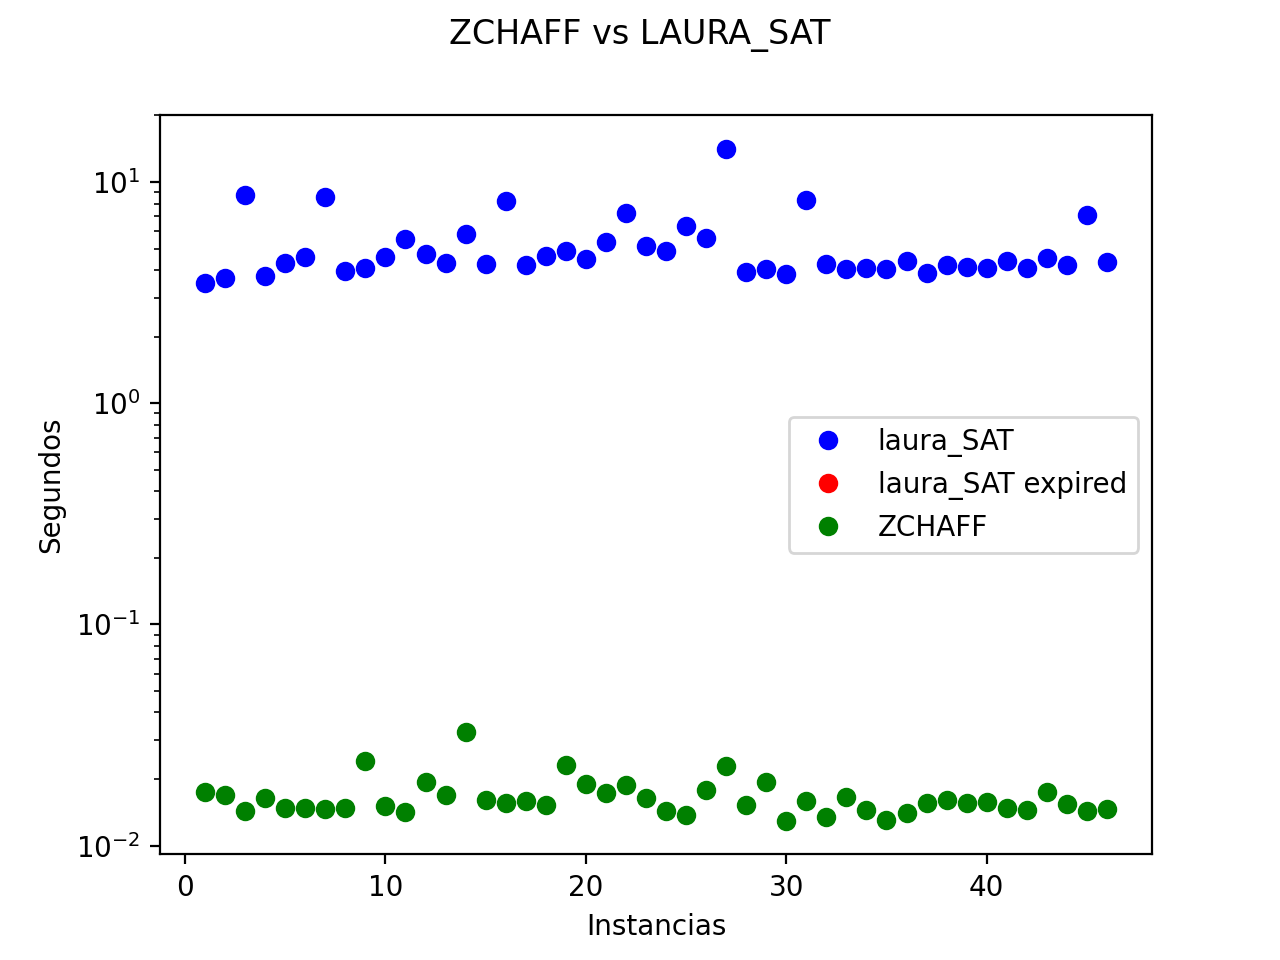
\includegraphics[scale=0.6]{Figure_1.png}\\

Donde el mayor tiempo que tuvimos fue de aproximadamente 12 segundos en la instancia 27, y en los demas problemas alcanzamos un promedio de 5 segundos de resolución. \\

Cuando se ejecute el programa, a través de la terminal se puede ver en tiempo real como se va resolviendo cada instancia del sudoku con nuestra implementación y a su vez también se observa la de ZCHAFF.\\

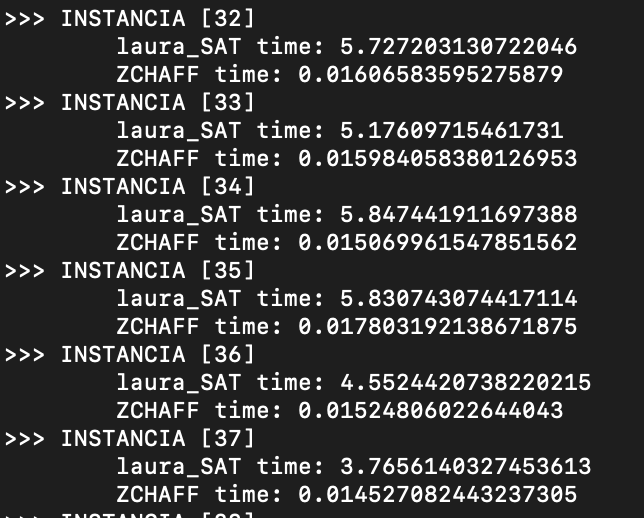
\includegraphics[scale=0.6]{Shell_Report.png}\\

En un archivo que por defecto nosotros llamamos \texttt{Soluciones.txt} se tendrán las soluciones en el mismo formato que se le pasó al programa. También creamos otro archivo llamado \texttt{Soluciones\_Matrices.txt} donde estarán los sudokus resuelto en forma matricial.\\

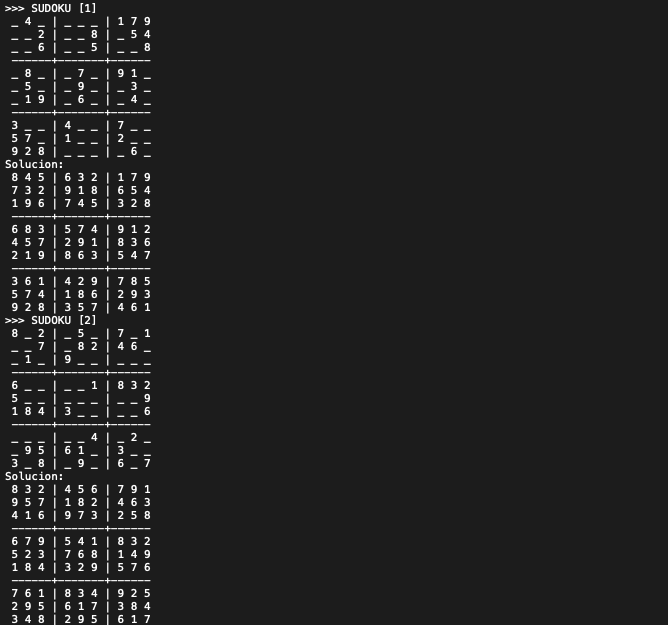
\includegraphics[scale=0.4]{Matrix_Solve.png}\\

\end{document}
